\documentclass[11pt,a4paper,spanish]{article}
\usepackage[spanish]{babel}
\usepackage[utf8]{inputenc}
\usepackage{times}
\usepackage{setspace} 
\usepackage{multicol}
\spacing{1.15}
\usepackage{hyperref}
\usepackage{array}
\usepackage{xurl}
\usepackage{graphicx}
\title{Análisis y riesgos de las tecnologías para lucha contra la Covid19.}
\pagestyle{myheadings}
\date{09/09/2021}
\author{Miguel Chacón Carrasco}
\usepackage{fancyhdr}
\pagestyle{fancy} 
\fancyhf{}
\lhead[\leftmark]{Miguel Chacón Carrasco}
\rfoot[]{\thepage} 
\renewcommand{\headrulewidth}{0pt}
\renewcommand{\footrulewidth}{0pt} 
\hoffset -1cm
\textwidth 15cm

\begin{document}
	\maketitle
\begin{tabular}{p{2cm} p{3cm} p{6cm} }
\textbf{Versión} & \textbf{Fecha} & \textbf{Comentarios}  \\
1              & 09-01-2021     & Primera versión.      \\
2              & 20-01-2021     & Corrección de errores      \\
3              & 22-01-2021     & Modificación del documento. Creación del anteproyecto.     \\
4              & 28-02-2021     & Marco legal.     \\
5              & 07-09-2021     & Integración de todo el desarrollo.     \\
6              & 09-09-2021     & Maquetación final. 
\end{tabular}
\begin{abstract}
Se ha planteado como proyecto de investigación los problemas que podría presentar el uso de las nuevas tecnologías en la privacidad de los datos y que efectos podría tener en la vida de los usuarios de estas tecnologías.

Se han desarrollado multitud de iniciativas para el control y recopilación de información para la lucha de la pandemia de COVID-19. Estas iniciativas recopilan multitud de información privada (geolocalización, resultados de pruebas médicas, inmunidad ante el virus, temperatura corporal, diagnósticos, contactos, pasaportes inmunitarios, control de confinamiento…) de los usuarios que pueden compartir o no con los gobiernos, centros de investigación y terceros.

Este trabajo se centra en investigar dichas iniciativas y nuevas tecnologías y hacer un estudio en profundidad de la efectividad contrastada para luchar contra el COVID-19, su situación legal en el mundo, la trasparencia de las soluciones (documentación y auditorias), la efectividad y precisión de la información que se da a los interesados, el control que tienen los usuarios de sus propios datos, tratamientos adicionales, los accesos por terceros y los riesgos que supone para los derechos y libertades de los individuos.
 
La información que recogen estas iniciativas puede suponer un riesgo, por ejemplo, para su trabajo, vida social, etc. en caso de que haya pasado el virus o no, en qué condiciones o si pueda tener secuelas de algún tipo. 

Para ello, se necesita hacer un estudio en profundidad de las iniciativas y del marco legal de las iniciativas, junto a la información que recogen para saber el impacto real en la sociedad.

\textbf{Palabras clave}: COVID-19, tecnologías, provacidad, geolocalización, datos

\end{abstract}

\section{INTRODUCCIÓN}
\subsection{CONTEXTO SANITARIO}
La COVID-19 es una enfermedad infecciosa causada por un virus de tipo coronavirus, de la familia del SARS que se detectó en Wuhan, en China, en diciembre de 2019. Esta enfermedad se propaga vía respiratoria, por pequeñas gotas de agua y saliva en suspensión el aire. También por contacto de mucosas, sistema respiratorio y ojos con material contaminado.

Las tasas de infección de esta enfermedad son superiores a otras conocidas, haciendo que la comunidad científica trabaje contrarreloj para buscar un método para frenar la propagación de la enfermedad.
El primer paciente registrado en España con COVID-19 se dio a conocer el 31 de enero del año pasado, en La Gomera. Sin embargo, como se indica en (Fita, 2020) la enfermedad pudo llegar mucho antes a España.

\subsection{CONTEXTO TECNOLÓGICO}
Actualmente la enfermedad afecta a todos los países del mundo, los cuales están tomando medidas para controlar la propagación.

Para reducir la propagación de la enfermedad, diferentes países, como es el caso de España, han destinado recursos a la implementación de nuevas tecnologías y aplicaciones para el control, rastreo y control de la enfermedad.

\section{ESTADO DE LA CUESTIÓN}
Para el desarrollo de la investigación se ha consultado posibles antecedentes en este tema. Por ello se buscan artículos de interés relacionados con el tema.

El artículo más parecido a este trabajo es el artículo (AGENCIA ESPAÑOLA DE PROTECCIÓN DE DATOS                                                                                                                                ), 2020b) de la bibliografía se expone un tema muy similar al de este trabajo.

En dicho artículo se exponen las bases y un pequeño análisis de los beneficios y costes a la privacidad de las siguientes tecnologías:

\begin{itemize}
\item Geolocalización mediante operadores de telecomunicaciones y en redes sociales
\item Aplicaciones, webs y chatbots para auto-test, como la aplicación CoronaMadrid de la Comunidad de Madrid, o cita previa
\item Aplicaciones de recogida de información de contagiados, como la aplicación Open-coronavirus.
\item Aplicaciones de seguimiento de contactos
\item Pasaportes digitales de inmunidad
\item Cámaras infrarrojas 
\end{itemize} 

En el artículo se llega a la siguiente conclusión: “hay que ser especialmente cuidadoso a la hora de tomar medidas que pueden tener consecuencias irreversibles y pueden estar guiadas únicamente por la urgencia, el miedo o, lo que es peor, otros intereses.” (AGENCIA ESPAÑOLA DE PROTECCIÓN DE DATOS (AEPD), 2020b)
\section{DESCRIPCIÓN DEL PROBLEMA}

En este trabajo se dispone a reunir y estudiar las diferentes tecnologías sacadas al público con el fin de luchar contra la pandemia del COVID-19, y mostrar si son eficientes o no en función de y frente a las políticas de privacidad y tratamiento de los datos, así como su legalidad dentro del marco normativo europeo. 

Esto es debido a que, con la rápida expansión de la enfermedad, se ha tenido que recurrir a nuevas tecnologías y fuentes de información para poder tener a dicha enfermedad bajo control y a la población lo más segura posible. Sin embargo, como se mostrará en el documento, muchas de las veces no se han hecho con las mejores políticas de datos o el mejor tratamiento. También, muchas de las veces, se han implementado tecnologías con mecanismos que no son los más apropiados o de la manera menos acorde a la legalidad vigente.

\section{DESARROLLO}
\subsection{MARCO LEGAL INTERNACIONAL}
Esta pandemia es a nivel mundial, y muchas de las propuestas nacen a nivel internacional. Uno de estos ejemplos es el llamado “Pasaporte Covid”, que muestra quien está vacunado y quien no, para poder viajar. Debido a esto, se debe mostrar el marco legal en el que se mueven el marco legal de dichas tecnologías y aplicaciones contra el Covid.
\subsubsection{MARCO LEGAL EUROPEO}
En parte nos basaremos en el reglamento europeo RGPD, ya que muchas de las aplicaciones parten de europea o afectan a ciudadanos de dicha región.

Este reglamento europeo afecta directamente a todos los países miembros de la Unión Europea, como es el caso de España.  Este establece las normas relativo a la protección de las personas físicas en lo que respecta al tratamiento de datos personales y a la libre circulación de estos datos. Las diferentes leyes que se desarrollen a nivel nacional tendrán que heredar todas las normas que se establecen en el reglamento RGPD, pudiendo ser ampliadas las normas que se establecen en dicho reglamento.

Por ello, cada tecnología o aplicación o tecnología tendrá que adaptarse a las leyes de cada país europeo, que usan como base el reglamento RGPD y, en caso de que no exista, se aplicará dicho reglamento.
\subsubsection{MARCO LEGAL EN ESTADOS UNIDOS}
En EE. UU., al ser un país tan federal, hay diferentes normas y estándares para el tratamiento de datos. Sin embargo, las leyes y estándares que afectan directamente a este proyecto son:

\begin{itemize}
\item \textbf{Estándar NIST 800-171}: establece una serie de reglas de buenas prácticas a seguir, muy parecido a los estándares ISO. Fue diseñado por el Instituto Nacional de Estándares y Tecnologías, organismo gubernamental para generar normas para las nuevas tecnologías. Estas normas influyen directamente en las aplicaciones y tecnologías desarrolladas para luchar contra la COVID.
\item \textbf{Ley de protección de la privacidad online de los niños (COPPA)}: ley creada para la protección de los datos de los menores de 13 años. Esto afecta directamente en aquellos casos en el que los infectados por la enfermedad posea una edad inferior a dicha edad.
\item \textbf{Ley CLOUD}: es el análogo a la RGPD, pero en territorio de EE. UU., siendo la última ley aprobada por EE. UU. Esta ley sienta las bases para que empresas americanas puedan firmar acuerdos de protección de datos con países miembro de la Unión Europea. Esta ley puede influir en aquellas tecnologías o aplicaciones que sean de empresas con sede en territorio de EE. UU. y sean utilizadas en regiones de la Unión Europea o que alguno de sus usuarios sea de la Unión
\end{itemize} 

\subsection{MARCO LEGAL NACIONAL}
La ley de Protección de Datos Personales y garantía de los derechos digitales (Jefatura del Estado, 2018) que establece los derechos del dueño de los datos y las obligaciones de los que tratan dichos datos.

Esta ley establece las siguientes obligaciones, que nos afecten de manera directa o indirectamente:

\begin{itemize}
\item Debe existir un consentimiento que, con carácter general, debe ser libre, informado, específico e inequívoco. Solo podrá existir consentimiento explícito en menores de edad si este tiene, como mínimo, catorce años. El consentimiento de los menores catorce años deberá darlo el titular de la patria potestad.
\item La aceptación se puede deducirse del silencio o de la inacción de los usuarios.
\item Toda brecha de seguridad que puedan afectar, directa o indirectamente, a los datos personales deben ser notificadas a la Autoridad de Control correspondiente en un plazo no superior a 72 horas.
\item Se han de adoptar medidas que garanticen de manera suficiente que están en condiciones de cumplir con las reglas, derechos y garantías que establece la ley.
\item Los interesados tienen derecho a no aportar documentos que ya se encuentren en poder de la Administración actuante o hayan sido elaborados por cualquier otra Administración.
\item Se define la figura del Delegado de Protección de Datos. A este se le atribuye su intervención en caso de reclamación ante las autoridades de protección de datos, de modo que el ciudadano pueda dirigirse a él.
\item Las Administraciones Públicas deberán recibir y recolectar todos los documentos electrónicamente mediante sus redes corporativas o mediante consulta a las plataformas de intermediación de datos habilitados a tal efecto.
\item En caso de fallecimiento del dueño de los datos, las personas vinculadas a dicho fallecido por razones familiares o designado como sus herederos podrán dirigirse al responsable o encargado del tratamiento al objeto de solicitar el acceso a los datos personales del fallecido y, en su caso, su rectificación o supresión (eliminación). Las personas o instituciones a las que el fallecido hubiese designado expresamente para ello podrán también solicitar el acceso a los datos personales de este y, en su caso su rectificación o supresión.
\end{itemize} 

Se establece que las siguientes aplicaciones y tecnologías:
\begin{enumerate}
\item Aplicaciones y tecnologías de geolocalización mediante operadores de telecomunicaciones y en redes sociales.
\item Aplicaciones y tecnologías de seguimiento de contactos.
\end{enumerate} 

Están sujetas a los artículos (22) Tratamientos con fines de videovigilancia, (25) Tratamiento de datos en el ámbito de la función estadística pública y (26) Tratamiento de datos con fines de archivo en interés público por parte de las Administraciones Públicas.

En los artículos (Gabinete Jurídico, 2020) y (AGENCIA ESPAÑOLA DE PROTECCIÓN DE DATOS (AEPD), 2020a) se exponen el informe jurídico y el estudio de las leyes, respectivamente.

“El tratamiento de categorías especiales de datos personales, sin el consentimiento del interesado, puede ser necesario por razones de interés público en el ámbito de la salud pública. Ese tratamiento debe estar sujeto a medidas adecuadas y específicas a fin de proteger los derechos y libertades de las personas físicas. […] Este tratamiento de datos relativos a la salud por razones de interés público no debe dar lugar a que terceros, como empresarios, compañías de seguros o entidades bancarias, traten los datos personales con otros fines.”  (Gabinete Jurídico, 2020)  

\subsection{HERRAMIENTAS INVESTIGADAS}
\subsubsection{TABLA RESUMEN DE HERRAMIENTAS DE ESTUDIO}

Las herramientas objeto de estudio son las siguientes:

\begin{tabular}{p{4cm} p{4cm}p{5cm}}
\textbf{Nombre} & \textbf{Desarrollador} & \textbf{Descripción}  \\ \hline
Radar covid              & Gobierno español.     & Aplicación para el seguimiento y detección de posibles positivos      \\ \hline
Certificado Digital covid              & Unión Europea     & Certificado a nivel europeo que indica la pauta de vacunación (dosis, tipo de vacuna, nombre de la vacuna), resultado de la última PCR, o si ha pasado el COVID o no.    \\ \hline
CoronaMadrid              & Comunidad de Madrid    & Aplicación de autodiagnóstico.     \\ \hline
AsistenciaCovid19              & Gobierno español    & Aplicación de autodiagnóstico.    \\ \hline
STOP COVID19 CAT              & Gobierno catalán     & Aplicación de autodiagnóstico.     \\ \hline
Aplicación de acceso a restauración en Castilla-La Mancha              & Gobierno Castilla la Mancha    & Aplicación para el rastreo mediante códigos QR     \\ \hline
MySOS              & Gobierno Nipón     & Aplicación médica con apartado relacionados con el COVID-19     \\ \hline
Tarjeta virtual sanitaria Madrid              & Comunidad de Madrid     & Aplicación médica que contiene una copia de la tarjeta sanitaria 
\end{tabular}

\subsubsection{RADARCOVID}
Esta es una aplicación móvil que permite avisar a los usuarios si han estado en contacto con una persona contagiada con COVID-19. Dicha aplicación fue desarrollada por el gobierno español y está disponible en Android y IOS. Usa la tecnología bluetooth para saber los contactos y en caso de que un usuario es positivo, debe indicarlo.

En sus políticas de seguridad se especifica que en ningún caso se almacenarán y/o tratarán los siguientes datos: (Gobierno de España, 2020c)

\begin{itemize}
\item En ningún caso los movimientos de los usuarios, excluyendo ciertas formas de geolocalización.
\item La dirección IP de los usuarios.
\item Los códigos de confirmación de positivo junto con otros datos personales de los usuarios.
\end{itemize}

Como parte del sistema de alerta de contactos de riesgo de la aplicación, se procesarán los siguientes datos de los usuarios que hayan dado positivo en el virus COVID-19 para el correcto funcionamiento de la aplicación.

\begin{itemize}
\item Unas claves de exposición temporal que el dispositivo del usuario ha generado los códigos aleatorios enviados a través del Bluetooth a los dispositivos con los que el usuario ha entrado conectado o en contacto, hasta un máximo de 14 días anteriormente. Se especifican que estas claves se suben al servidor de la aplicación para que otras aplicaciones puedan tener accesos a estas claves. Sin embargo, estas claves no guardan relación alguna con la identidad del usuario.
\item Un código de confirmación de un solo uso de 12 dígitos facilitado por los sanitarios al usuario en caso de una prueba positiva. Este código debe ser introducido por el usuario en la aplicación para permitir que se cargue al servidor de las claves de exposición temporal de manera voluntaria.
\item En caso de que aplique, el consentimiento del usuario, para el envío de claves de exposición temporal a los responsables europeos para su tratamiento en aplicaciones de contacto.
\item El aviso de notificación de contacto, con el objetivo de recoger estadísticas anónimas y agregarse el volumen de notificaciones que produce en el sistema.
\end{itemize}

La legislación en la que se basa esta aplicación es la siguiente:

\begin{itemize}
\item Reglamento (UE) 2016/679, de 27 de abril de 2016.
\item Ley Orgánica 3/2018, de 5 de diciembre, de Protección de Datos Personales y garantía de los derechos digitales.
\item Ley Orgánica 3/1986, de 14 de abril, de Medidas Especiales en Materia de Salud Pública.
\item Ley 33/2011, de 4 de octubre, General de Salud Pública.
\item Ley 14/1986, de 25 de abril, General de Sanidad.
\item Real Decreto ley 21/2020, de 9 de junio.
\item Acuerdo de 9 de octubre de 2020, entre el Ministerio de Asuntos Económicos y Transformación Digital y el Ministerio de Sanidad acerca de la aplicación “Radar COVID”.
\end{itemize}

\subsubsection{CERTIFICADO DIGITAL COVID}
Se trata de un sistema de certificación que muestra que un ciudadano de un país europeo cumple con al menos una de las siguientes:

\begin{itemize}
\item ha recibido la pauta completa de vacunación de cualquiera de las vacunas contra la COVID-19 aprobadas por la Unión Europea.
\item se ha realizado una prueba de detección del COVIS-19 cuyo resultado ha sido negativo
\item se ha recuperado totalmente de la enfermedad COVID-19
\end{itemize}

\begin{figure}[h!]
  \centering
  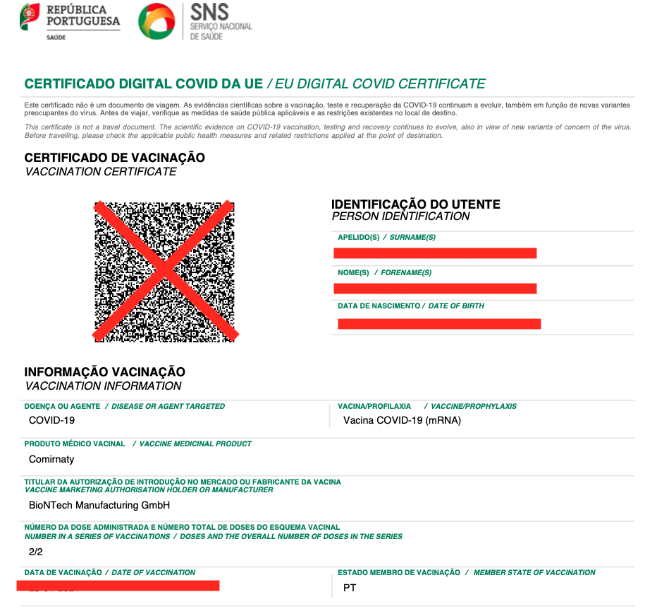
\includegraphics[width=0.65\linewidth]{1.png} 
  \caption{Ejemplo pasaporte CERTIFICADO DIGITAL COVID}
\end{figure}
Sus principales características son:

\begin{enumerate}
\item puede estar en formato digital o en papel
\item posee un código QR identificativo
\item es totalmente gratuito
\item disponible en la lengua nacional y en inglés
\item hecho basándose en la seguridad y fiabilidad 
\item válido para todos los países de la UE y terceros países que se han acogido a este
\end{enumerate} 

Los países no europeos en los que está disponible son:

\begin{enumerate}
\item Islandia
\item Liechtenstein
\item Noruega
\item San Marino
\item Suiza
\item Vaticano
\end{enumerate}

El pasaporte covid entró en vigor el 15 de junio de 2021, el mismo día de su publicación en el Diario Oficial de la Unión Europea, y será aplicable desde el día 1 de julio de 2021 hasta el día 30 de junio de 2022.

El funcionamiento del certificado es el siguiente:

\begin{enumerate}
\item El certificado contiene un código QR con una firma digital para protegerlo contra una posible falsificación.
\item Cuando se comprueba el certificado, se escanea el QR y se verifica dicha firma.
\item Cada emisor (por ejemplo: un hospital, un centro de salud, una autoridad sanitaria, etc) tiene su propia firma digital. Esta información se almacena en una base de datos segura en cada país miembro o no miembro que se haya acogido.
\item La Unión Europea ha creado un portal a través del cual se pueda verificar las firmas de los certificados en todos los países acogidos. Los datos personales del titular del certificado se tramitarán a través del portal. La UE también ayudó a los estados miembros a desarrollar el software y las aplicaciones necesarias para expedir, almacenar y verificar los certificados y gestionó las pruebas necesarias para que dichos estados miembros se unieran al portal.
\end{enumerate}

\textbf{¿Cómo se tratan los datos personales?}

La propia Unión Europea establece lo siguiente:“Dado que los datos que hay en los certificados incluyen información médica personal sensible, la UE garantizará un “nivel de protección de datos muy elevado” (Comisión Europea, 2021).

Los certificados solo tendrán que contener la información mínima y necesaria, además de que los países que hacen uso de este certificado no podrán conservar esta información. Para hacer la comprobación, se gestionará únicamente la validez y autenticidad del certificado y los datos, comprobando la identidad de quien lo haya expedido y firmado. Durante dicho proceso no se intercambian ni guardan datos personales. Todos los datos sanitarios seguirán perteneciendo al estado miembro que haya emitido el certificado.

El sistema de emisión y gestión de los certificados no necesita la creación y el mantenimiento de una base de datos de los certificados sanitarios a escala de la UE y no se mandará ningún dato personal a través de la pasarela de la UE y de ningún otra.

\textbf{¿Por qué se acepta este certificado?} Porque según el artículo 5.5 del Reglamento Europeo 2021/953 “cuando los Estados miembros acepten pruebas de vacunación con el fin de no aplicar las restricciones a la libre circulación establecidas, de conformidad con el Derecho de la Unión, para limitar la propagación del SARS-CoV-2, también aceptarán, en las mismas condiciones los certificados de vacunación expedidos por otros Estados miembros de conformidad con el presente Reglamento” (Parlamento Europeo, 2021).

\subsubsection{HERRAMIENTAS AUTOTEST}
\textbf{CoronaMadrid}

\begin{figure}[h!]
  \centering
  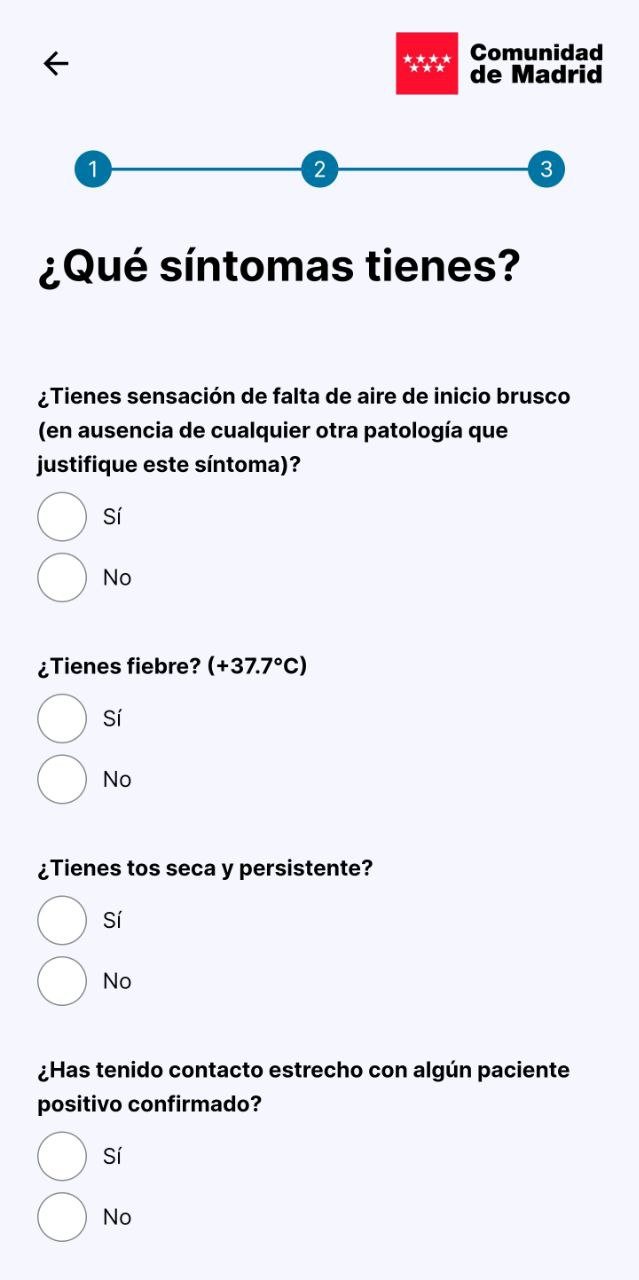
\includegraphics[width=0.35\linewidth]{2.png} 
  \caption{Autotest de CoronaMadrid}
\end{figure}

Esta aplicación fue lanzada por la Comunidad de Madrid para el autodiagnóstico a través del teléfono móvil y saber si tienes síntomas compatibles con el COVID-19. Según la propia página de la Comunidad de Madrid: “Esta nueva herramienta hace posible que cualquier ciudadano, desde su domicilio, pueda acceder y consultar cuestionarios en los que se irán examinando los síntomas de coronavirus y las posibles dolencias que podrían tener.”

La aplicación se incorpora al entorno de aplicaciones que posee la Comunidad de Madrid para el tema salud (como son la tarjeta sanitaria, cita sanitaria, ...).

Para poder acceder a la aplicación móvil es necesario o bien tener instalado la app de la tarjeta sanitaria o bien a través de los datos de la tarjeta sanitaria. 

Para la gestión de los datos se valen del sistema de credenciales de la aplicación de la Tarjeta Sanitaria, guardando el identificador del usuario (en este caso, el CIPA del usuario, que es el número de la tarjeta de salud) gestionando todos los datos a través de la infraestructura y encriptación de la Comunidad de Madrid (como la carpeta virtual sanitaria o similares). Por otro lado, también nos pide acceso a nuestro número de teléfono y a nuestra ubicación GPS, según la política de seguridad para "saber dónde te encuentras para poder ofrecerte las mejores medidas preventivas y de evaluación".

Sin embargo, en su página web, a través de la cual también podemos realizar el autotest, nos pide el número de teléfono y la ubicación.
En conjunto, la aplicación trata los siguientes datos 

\begin{itemize}
\item Nombre completo y apellidos.
\item Número de teléfono móvil al que se enviará un SMS de verificación en el momento del registro.
\item DNI / NIE para cruzarlo con la tarjeta sanitaria.
\item Fecha de nacimiento, con objeto de poder establecer el grupo de población en el que te encuentras. Esto ayuda a saber si estás en un grupo de riesgo y a la ponderación de los posibles síntomas.
\item Dirección completa, con código postal y comunidad autónoma en la que se encuentra el usuario.
\item Género.
\item Geolocalización, que se establece como opcional y se hará mediante el GPS del teléfono. Según las políticas de privacidad “Sólo se utilizará a la hora de registrarte y realizar tus autoevaluaciones, y únicamente en el caso de que des tu autorización para ello”.
\item Los datos de salud obtenidos con la autoevaluación dependiendo de los síntomas que se hayan experimentado e indicado. Más específicamente, datos como si se ha tenido más de 37,7ºC de fiebre, tos seca, contacto estrecho con un positivo, ...
\end{itemize}

\begin{figure}[h!]
  \centering
  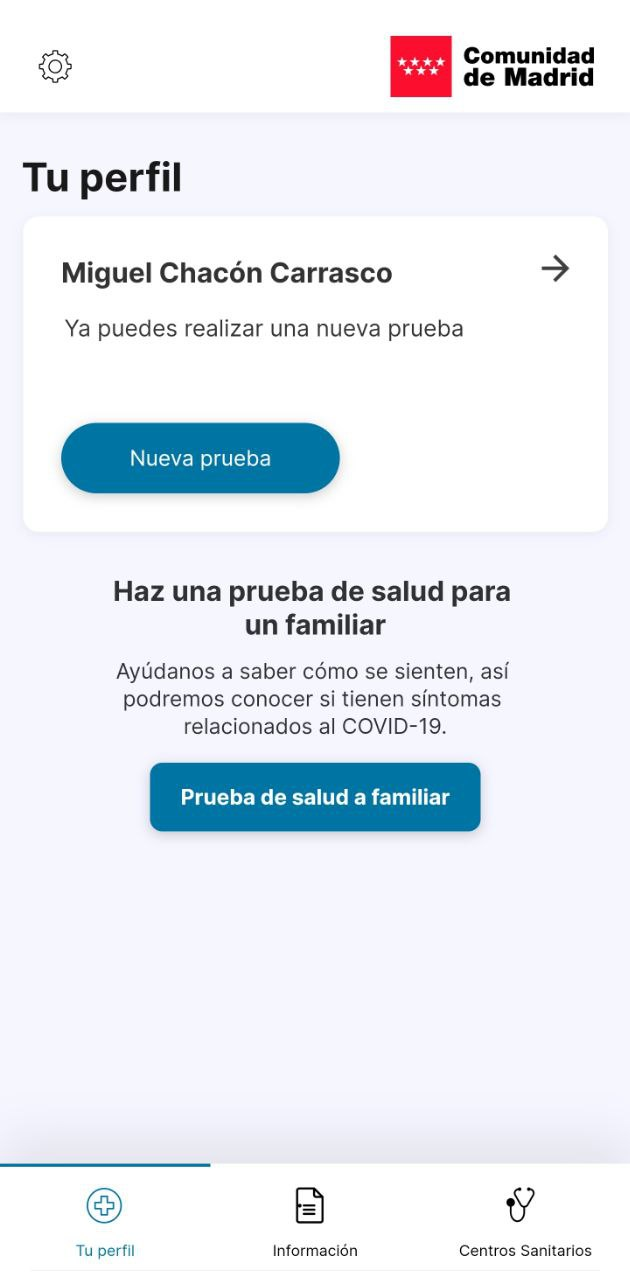
\includegraphics[width=0.45\linewidth]{3.png} 
  \caption{Página inicial de CoronaMadrid}
\end{figure}

Todos estos datos se recogen con los siguientes fines:

\begin{enumerate}
\item para temas estadísticos;
\item para investigación;
\item para archivo por el interés global
\end{enumerate}

Y, todo según las políticas de seguridad, estos datos se guardarán mientras sean necesarios para los fines establecidos en el punto anterior. Sin embargo, mientras estos datos se guarden, se hará de manera anónima.

Se indica que las personas que tienen acceso a los datos son:

\begin{enumerate}
\item Los profesionales sanitarios, para que se pongan en contacto directamente con el usuario en caso de que la aplicación haya dado un posible positivo.
\item Cuando la requieran las Autoridades, nacionales y/o internacionales, con las que sea necesario compartir la información. En ese caso, se verificará siempre la legitimidad de dichas solicitudes y se garantizará se ajustan a la normativa vigente.
\item Los proveedores y colaboradores, así como a las empresas que estos subcontraten para este fin.
\end{enumerate}

\textbf{AsistenciaCovid19}

Esta es una aplicación web y móvil para las comunidades autónomas que no poseen una aplicación regional de autodiagnóstico de covid. Estas regiones son: Canarias, Cantabria, Castilla La Mancha, Extremadura, Islas Baleares y Región de Murcia.

Los datos obtenidos son los siguientes:

\begin{itemize}
\item Nombre y apellidos del usuario
\item Número de teléfono móvil, para la notificación vía SMS
\item DNI, para el cruce con los datos sanitarios del usuario
\item Dirección completa y código postal
\item Fecha de nacimiento, para poder establecer el grupo de población en el usuario está y así poder ponderar los síntomas.
\item Geolocalización (para teléfonos móviles se usará el GPS)
\item Género (opcional).
\item Datos de salud relacionados con los síntomas que el usuario tiene.
\end{itemize} 
\newpage
\begin{figure}[h!]
  \centering
  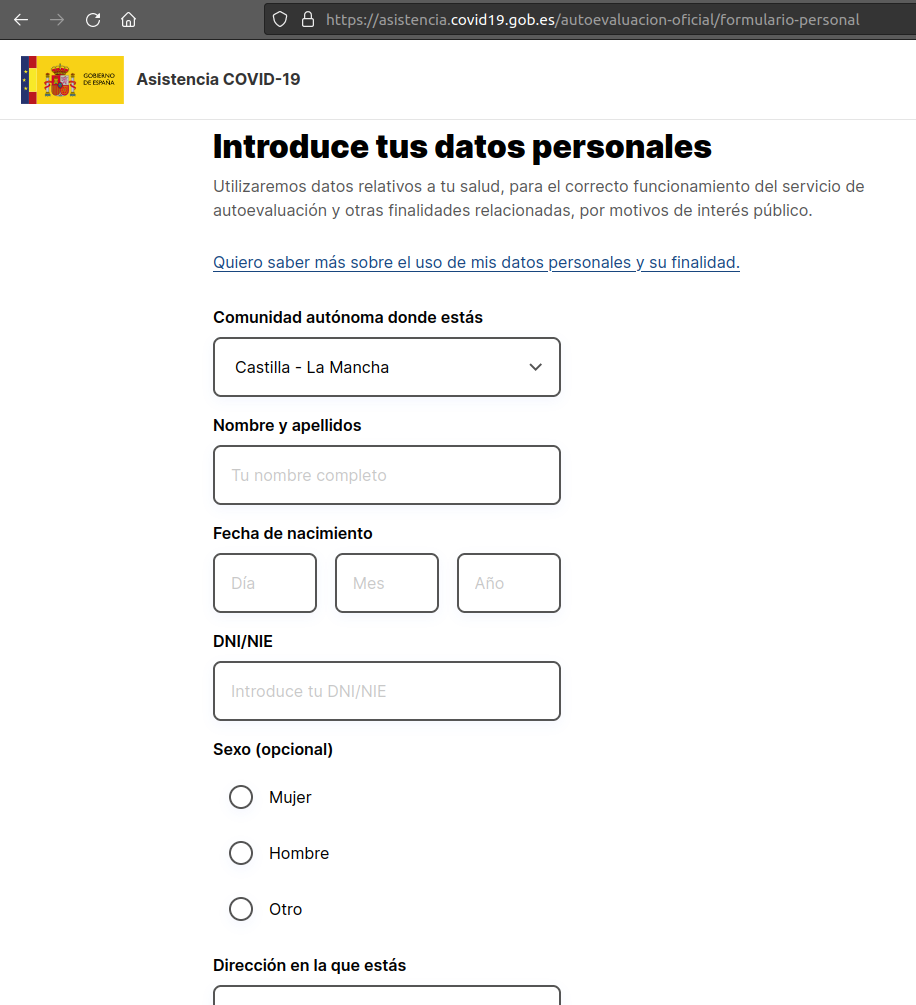
\includegraphics[width=0.55\linewidth]{4.png} 
  \caption{AsistenciaCovid19}
\end{figure}

Su similitud es casi total a la aplicación CoronaMadrid, siendo los datos que recoge son los mismos y su interfaz y tratamiento son prácticamente iguales.

Las políticas de seguridad (Gobierno de España, 2020b) son exactamente iguales a la de la aplicación CoronaMadrid, con lo que los resultados y opiniones son iguales a dicha aplicación. Lo único diferente es la publicación en el BOE en la que se publica el “Convenio entre la Secretaría de Estado de Digitalización e Inteligencia Artificial y la Comunidad Autónoma de Extremadura, sobre la adhesión al uso de la Aplicación AsistenciaCOVID19” (Boletin Oficial del Estado, 2020). En él, se establece que se establece el tratamiento de datos en esa Comunidad autónoma. Lo más resaltable de este BOE son los siguientes:

\begin{itemize}
\item El apartado del Deber de Secreto: donde se especifica que harán en ambas partes (Estado y Comunidad Autónoma de Extremadura)
\item Duración, resolución y extinción del convenio redactado en dicho BOE
\item Modificación general del tratamiento de datos
\end{itemize}

\textbf{STOP COVID19 CAT}

Esta es la aplicación de autotest de Cataluña, estando exclusiva para teléfonos móviles, estando sus políticas de privacidad exclusivamente desde dentro de la aplicación y también en la página web. Sin embargo, están explicados con mayor detalle dentro de la aplicación.

Esta aplicación sigue la misma estructura que las dos anteriores en tema de políticas de privacidad. Los datos recogidos por esta aplicación son los siguientes:

\begin{itemize}
\item Datos identificativos (CIP o DNI, Edad, Sexo, Nombre completo y dirección)
\item Datos de contacto (teléfono móvil y teléfono alternativo)
\item Todos los datos de salud obtenidos en el autotest, que no se almacena en el móvil, sino que se envían directamente al servidor
\item Datos de localización. Esta opción es opcional, pero si se ha activado esta opción, se recogerá también.
\item De manera opcional, se recogen también las notificaciones push.
\end{itemize}

\begin{figure}[h!]
  \centering
  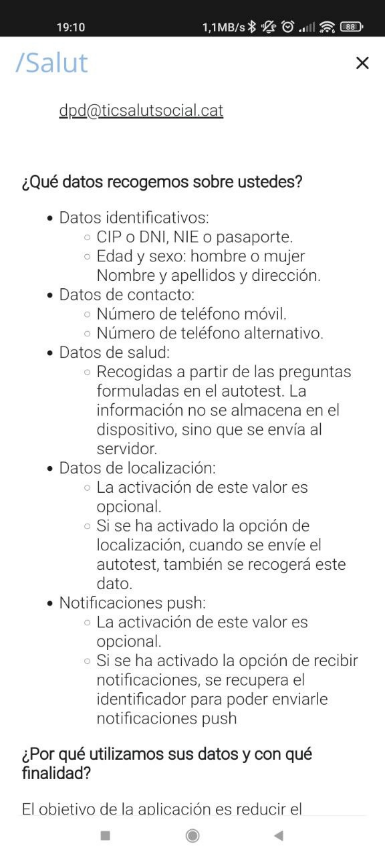
\includegraphics[width=0.35\linewidth]{5.png} 
  \caption{Datos STOP COVID19 CAT}
\end{figure}

El resto de las políticas, aunque con más detalle, son iguales al resto de aplicaciones de autotest. Se establece el encargado de tratamiento de los datos y, en cuanto a quién tendrá acceso y durante cuánto tiempo, se especifica exactamente lo mismo que en las aplicaciones como CoronaMadrid, que pueden acceder terceros, incluido subcontratados.

\textbf{Resto de aplicaciones autotest en España}

Las aplicaciones de autotest oficiales restantes, por comunidades autónomas, son:

\begin{enumerate}
\item SaludResponde en Andalucía
\item Salud Informa en Aragón
\item SACYL CONECTA en Castilla y León
\item CoronaTest Navarra en la Comunidad Foral de Navarra
\item GVA Coronavirus en la Comunidad Valenciana
\item COVID-19.eus en el País Vasco
\end{enumerate} 

Estas aplicaciones las agrupo en una misma sección porque siguen el mismo patrón. Todas recogen los mismos datos, similares a las anteriores aplicaciones de autotest. Estos datos son:

\begin{itemize}
\item Nombre completo
\item DNI o CIPA
\item Localización
\item Dirección
\item Teléfono
\item Datos de salud
\end{itemize}

También es reseñable que, en todas estas aplicaciones, el acceso a las políticas de privacidad es difícil de acceder, teniendo incluso en alguna de ellas descargar la aplicación para poder acceder a ellas. También, en otras se encuentran desestructuradas y resumidas, proporcionando información superficial.

Lo único que cambia entre las políticas de privacidad es la persona encargada del tratamiento, ante quien ejecutar los derechos y datos dentro de la prueba en sí (a partir de qué valor se considera fiebre, por ejemplo).

Por otro lado, el tratamiento en sí de los datos es igual entre estas aplicaciones, pareciendo una copia una de otras. Todas envían los datos directamente al servidor, sin guardarlo en el dispositivo. También, estos datos se usarán para fines médicos, de investigación y estadísticos. Unido a esto, se suma que podrán acceder a los datos las autoridades médicas y los terceros que estime cada comunidad autónoma.

\subsubsection{Aplicación de acceso a restauración en Castilla-La Mancha mediante QR}

La aplicación es Ocio Responsable en CLM, que tiene como objetivo poder acceder de manera segura a locales de ocio de la comunidad autónoma mediante el uso de códigos QR identificativos. Esta aplicación es totalmente voluntaria y sirve para poder identificar a los usuarios que hayan estado en contacto en caso de que haya un positivo.

\begin{figure}[h!]
  \centering
  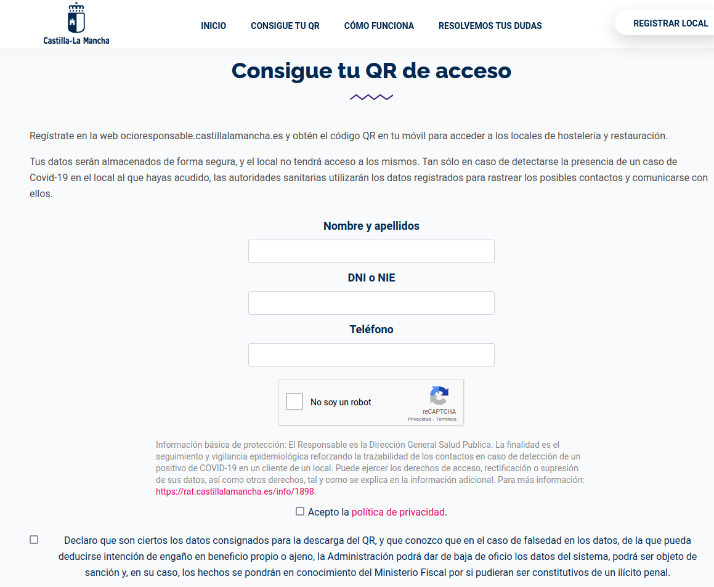
\includegraphics[width=0.80\linewidth]{6.png} 
  \caption{Ocio Responsable Castilla la Mancha}
\end{figure}

Para ello, tanto ciudadanos como locales se deben registrar en la aplicación, pudiendo el ciudadano generar un código QR y los locales leer dichos códigos QR.

En caso de que un positivo COVID haya coincidido con el usuario en un determinado local, un profesional sanitario usará los datos de la aplicación, guardados en el código QR, para llamar al usuario e iniciar el rastreo.

Los datos introducidos en la aplicación son “los mínimos imprescindibles para el correcto desempeño de la aplicación”, según sus políticas de privacidad. Además, en el momento en el que se use el código QR en un local, los datos son confidenciales y se borrarán a los 28 días, tras lo cual se anonimiza para fines estadísticos. También se define como contacto estrecho aquel en el que coinciden personas sin mascarilla durante más de 15 minutos.

Los datos no son visualizados directamente por los locales, permitiéndole usar el DNI en lugar del código QR. Esto es debido a que te pide los siguientes datos:

\begin{itemize}
\item Nombre
\item DNI
\item Teléfono
\end{itemize}

Una vez rellenado esto, como ciudadano, se te envía vía SMS un código QR como el siguiente:

\begin{figure}[h!]
  \centering
  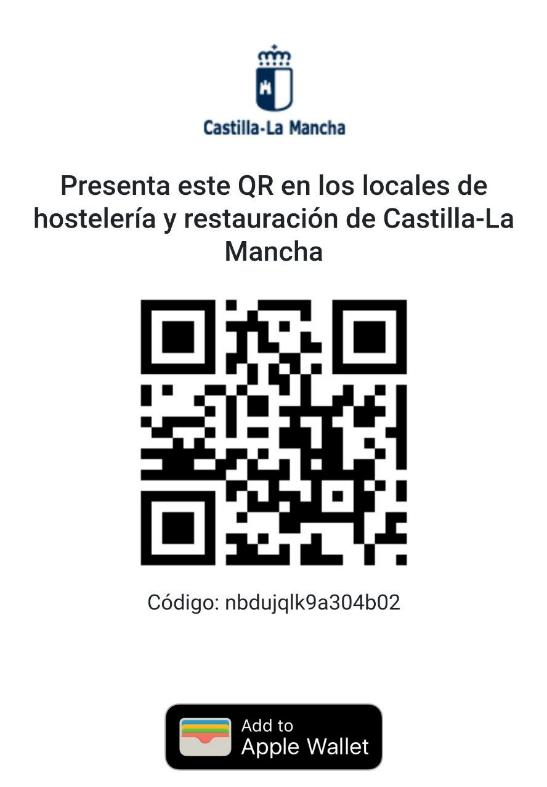
\includegraphics[width=0.45\linewidth]{7.png} 
  \caption{QR Ocio Responsable Castilla la Mancha}
\end{figure}
Para los locales se tiene que registrar a través de la web, mediante el siguiente formulario, y usar posteriormente la app móvil para leer los códigos QR.

\begin{figure}[h!]
  \centering
  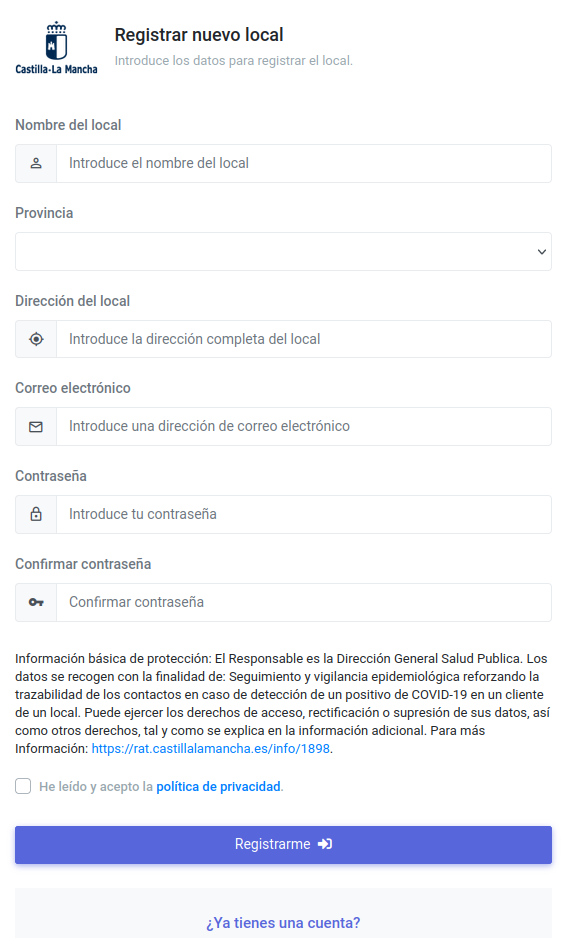
\includegraphics[width=0.45\linewidth]{8.png} 
  \caption{Registro Locales Ocio Responsable}
\end{figure}

\newpage
\subsubsection{APLICACIONES MÉDICAS}
\begin{figure}[h!]
  \centering
  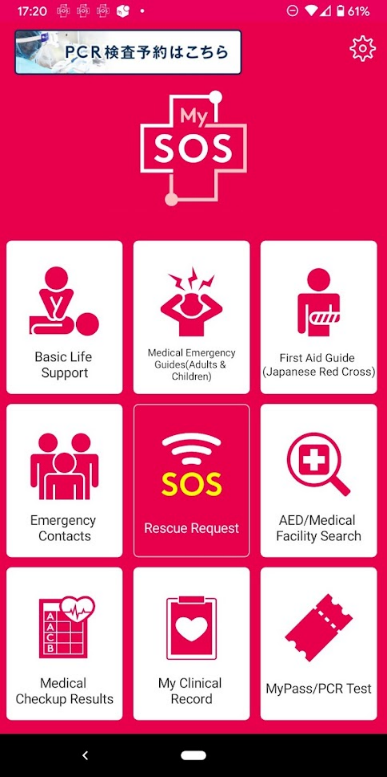
\includegraphics[width=0.35\linewidth]{9.png} 
  \caption{MySOS}
\end{figure}

En este apartado usaremos como ejemplo la aplicación MySOS como ejemplo, pues todas son muy similares. Esta aplicación está disponible tanto para IOS como para Android.


Este tipo de aplicaciones se han actualizado para introducir apartados relacionados con el covid, además de apartados como emergencias médicas, chequeos y similares unificados en una misma aplicación. 
La cuestión es que, en el mundo digitalizado e interconectado de hoy en día, las políticas de privacidad de estas aplicaciones se han vuelto enormemente importantes, pues se hacen acorde a la legislación del país donde se desarrollan. 

En el ejemplo que nos ocupa, es una aplicación de origen japonesa y en sus políticas de privacidad (ALLM, 2020) se especifica que recogen los siguientes datos:

\begin{enumerate}
\item Datos de salud y fitness almacenados en el dispositivo
\item Datos de localización (GPS)
\item Información de contacto
\item Datos de usuario
\item Identificadores
\item Datos de uso
\end{enumerate} 

Otro ejemplo es la aplicación de tarjeta virtual de la Comunidad de Madrid. Esta aplicación, que fue diseñada inicialmente como un sustituto de la tarjeta sanitaria física.

Con la pandemia, la Comunidad de Madrid decidió añadir apartados y funcionalidades destinados para la lucha contra el COVID. Estos apartados son los siguientes:

\begin{itemize}
\item “Mis pruebas diagnósticas COVID”, que te permite acceder a todos los diagnósticos del usuario.
\item “Carnet Vacunación Frente a SARS-Cov-2”, como pequeño resumen de la pauta de vacunación del usuario.
\item “Autocita Vacuna COVID”, pequeña funcionalidad que permite que los usuarios se citen para vacunarse, eligiendo fecha, franjas horarias y centro de vacunación si hubiera posibilidad. Esto agiliza el trámite de vacunación en gran medida.
\item “Certificado Covid Digital de la UE”, es una funcionalidad que te permite acceder y descargar el certificado digital, además de certificado de una prueba o un certificado de recuperación de la enfermedad en caso de que estuvieran disponibles.
\item Apartado para abrir la app CoronaMadrid.
\end{itemize} 

Todos los datos de la aplicación son obtenidos de los servidores del sistema de salud de la Comunidad de Madrid, mediante el código CIPA de la tarjeta sanitaria. Para habilitar esta aplicación y por motivos de seguridad, se tiene que llamar a un teléfono creado por la Comunidad de Madrid para un doble factor de autenticación. Después de esta llamada, se envía un código de autentificación para poder registrarse. Una vez realizado esto, el usuario estará registrado y todas las consultas se hacen usando el código CIPA. La aplicación te pide permiso para el acceso a los datos médicos que se muestran en la aplicación. Esto se puede ver en los datos de protección de datos (Comunidad de Madrid, 2020b) y se puede observar los diferentes reglamentos y leyes de protección de datos:

\begin{enumerate}
\item Ley Orgánica 3/2018, de 5 de diciembre, de Protección de Datos Personales y garantía de los derechos digitales.(Gobierno de España, 2018)
\item REGLAMENTO (UE) 2016/679 DEL PARLAMENTO EUROPEO Y DEL CONSEJO de 27 de abril de 2016
\end{enumerate} 

Estas dos leyes son importantes ya que son datos médicos, que se deben de tratar con el mayor cuidado y el mayor de los mecanismos de protección. 

En cuanto a los datos que utiliza son los mínimos para consultar que el usuario pide, y siempre con doble factor de autenticación. Además de que nada se almacena en el dispositivo móvil y todas las comunicaciones se hacen usando los mayores estándares de seguridad.

\section{Resultados}
\subsection{RADARCOVID}
Según la página oficial de la aplicación (Gobierno de España, 2020a), ha habido aproximadamente 7617983 descargas hasta julio, lo que supone algo más del 18\% de la población española, suponiendo que cada una de esas descargas corresponda a una sola persona. Esto plantea el primer problema, pues al menos un 60\% de la población debía utilizarla para que el rastreo de contactos fuera efectivo según un estudio de la Universidad de Oxford (OXFORD UNIVERSITY, 2020). Además, según los propios datos de la página de la aplicación, solo 8 de cada 100 casos se vuelcan en la aplicación.

\begin{figure}[h!]
  \centering
  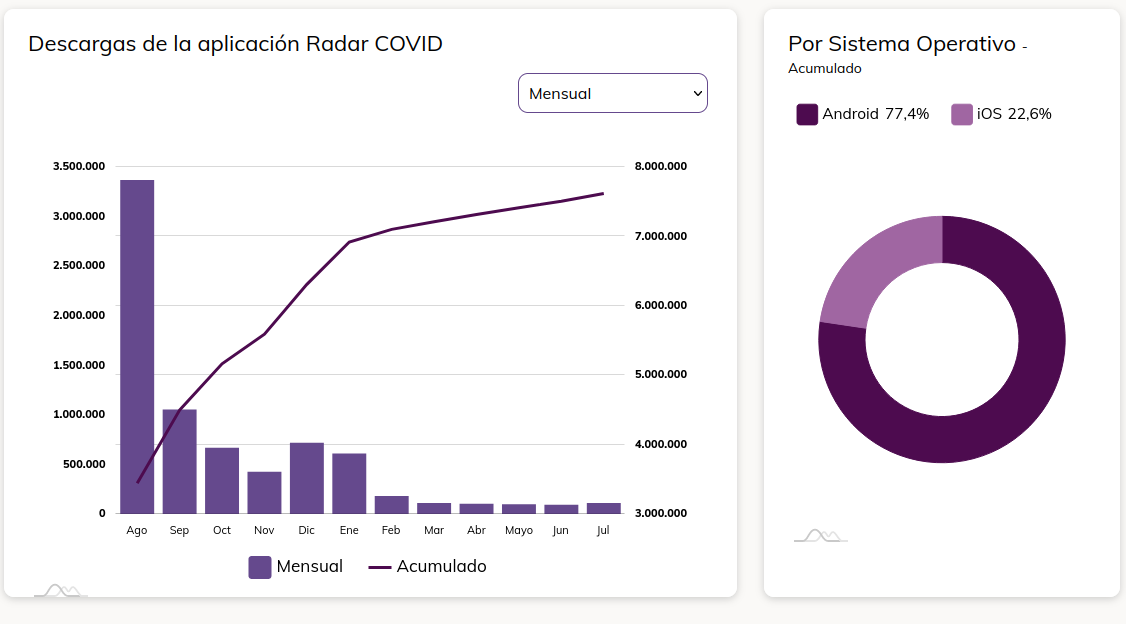
\includegraphics[width=0.85\linewidth]{11.png} 
  \caption{Gráfica de descargas RadarCOVID}
\end{figure}
Otro factor son los diferentes procedimientos, incluyendo por incumplimiento de RGPD, hacia la aplicación Uno de ellos es la irregularidad a la hora de hacer público el código fuente de la aplicación de manera accesible y clara, debido a que, aunque estaba la aplicación disponible desde junio de 2020, el código no estaba disponible hasta septiembre de 2020.

En otra demanda, presentada en septiembre de 2020, se solicita a la AEPD que analice si la aplicación cumplía “con los principios de licitud, lealtad, transparencia y responsabilidad proactiva (Art.5 RGPD)” (Enseñat, 2020). Esto debido a que la SGAD no había publicado la Evaluación de Impacto sobre la Protección de Datos (EIPD), como pedía expresamente el Comité Europeo de Protección de Datos.
  
Por otra parte, el Comité Europeo de Protección de Datos sacó una serie de directivas para el correcto desarrollo e implementación de aplicaciones como esta. En ellas se especifica la evaluación de impacto de las aplicaciones “relativa a la protección de datos antes de su despliegue” (Comité Europeo de Protección de Datos, 2021).

Desde el punto de seguridad, el 9 de octubre de 2020 se detectó una vulnerabilidad de seguridad. Esta vulnerabilidad es causada por el hecho de que las conexiones de la aplicación con los servidores (la subida de la información del positivo) sólo las hacen los casos positivos. Por tanto, cualquiera que esté en el camino de los datos con la capacidad de monitorizar el tráfico entre la aplicación y los servidores podría identificar qué usuarios tienen la enfermedad. Aunque este parche ha sido corregido mediante el envío de tramas falsas, sin embargo, debido a que el proveedor de la nube es Amazon y una vulnerabilidad con esta red, se podría diferenciar entre la comunicación verdadera y las falsas.

También está la cuestión de la localización y el Bluetooth en Android. En algunos casos, la app en teléfonos de base Android, el sistema operativo más usado en móviles, te pide que actives la localización para que el Bluetooth pueda funcionar. Google justificó esto en base a que desde 2015 y en todas las versiones superiores a Android 6.0, es necesario que esté la localización activa para utilizar cualquier aplicación de este tipo, no sólo la de RadarCovid.

\subsection{CERTIFICADO COVID}

Diferentes comunidades autónomas decidieron implementar el Certificado Covid para el acceso al ocio nocturno, como es Cantabria o Galicia. En la gran mayoría fueron rechazados por los tribunales. 
Esto es debido a que, tomando como ejemplo Galicia, el anómalo proceder por parte de la Xunta de Galicia indujo a confusión, por lo que no se ha sometido al control adecuado. Este control se debe hacer porque se trata de una norma que limita y controla los derechos de movilidad.

También, diferentes tribunales establecen que usar el Certificado COVID-19 implicaría mostrar datos protegidos por la constitución y obligaría a los hosteleros a tener un tratamiento de datos sensibles.

Por otro lado, el Tribunal Europeo de Derechos Humanos ha señalado que “el respecto al carácter confidencial de la información sobre la salud constituye un principio esencial del sistema jurídico de todos los Estados parte en la Convención”.

Por otra parte, la Agencia Española de Protección de Datos, el día 30 de julio de 2021, requirió a varias comunidades autónomas información sobre el uso del certificado de vacunación incluido en el certificado COVID para el acceso a establecimientos de ocio. En este caso, se ha requerido información a las consejerías de salud de Galicia y Canarias para ver la legalidad del tratamiento de los datos y su base legal. Como se indica en el requerimiento “La utilización para estos fines de certificados acreditativos de la situación sanitaria en relación con la COVID-19 implica la necesidad de contar con una base legal apropiada[...]” (AGENCIA ESPAÑOLA DE PROTECCIÓN DE DATOS (AEPD), 2021). Esto es debido a que no solo se deben tener en cuenta el tratamiento de los datos, sino que, como indica la AEPD, parte de la población no ha tenido acceso a la vacunación en el momento en el que se sacó la propuesta.

\subsection{HERRAMIENTAS DE AUTOTEST}

\subsubsection{CORONAMADRID}

Resulta curioso que, aunque piden solo los datos “estrictamente necesarios” según la página web, el DNI y localización, entre otros, sea necesario para hacer un autotest, cuando debería de ser totalmente voluntario. Después de la salida de la aplicación, sacaron una página de preguntas frecuentes en donde se indica respecto a datos como el DNI que "es opcional y servirá para un mejor procesado de los datos por las Autoridades competentes” (Comunidad de Madrid, 2020a) y en cuanto al número de teléfono “resulta menos intrusivo para garantizar que el mayor número posible de personas tenga acceso al servicio”. Sin embargo, tal y como está diseñada la aplicación, no parece así, llegando a ser que sea cuestionable que sea obligatorio el hecho de tener que ingresar el teléfono móvil.

\begin{figure}[h!]
  \centering
  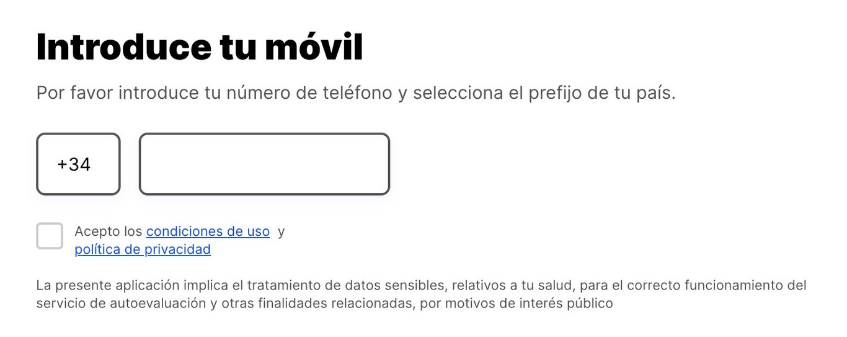
\includegraphics[width=0.7\linewidth]{12.png} 
  \caption{Teléfono CoronaMadrid}
\end{figure}

Por otro lado, en cuanto a las dudas de la geolocalización, la Comunidad de Madrid indica que “el usuario puede voluntariamente optar o no por aceptar la geolocalización”, sin embargo, el hecho de que lo pida hace preguntar para qué y cómo se trata dicho dato.

En cuanto al borrado de datos, se indica que “Una vez se satisfagan esas finalidades los datos son borrados o anonimizados". Esto supone un problema a la hora de privacidad, ya que se podría generar filtraciones de datos personales y el usuario no sabe realmente cuándo serán borrados los datos o si serán realmente borrados. También, al no disponer del código fuente, no se puede comprobar el destino de los datos, así como su propia integridad o el envío seguro de dichos datos.

Por último, comentar el tratamiento de datos con terceros indicados en las políticas de seguridad. En ningún punto de las páginas de la aplicación, incluido las propias políticas de seguridad, se establece quienes son, los datos que reciben, los tratamientos que van a hacer ni la explicación de cómo se va a pasar los datos.

\subsubsection{ASISTENCIACOVID}

Los resultados son los mismos de la aplicación anterior. Realmente no varía ni siquiera el valor a partir del cual se considera fiebre. Lo único que varía es la entidad de tratamiento de datos y la persona encargada del tratamiento de los datos obtenidos. 

Con lo que mi conclusión es la misma que para la aplicación de CoronaMadrid, siendo una cantidad de datos pedidos por una aplicación de autotest, totalmente voluntaria.

\subsubsection{STOPCOVID19 CAT}

Esta aplicación recoge muchos más datos que las anteriores, teniendo el mismo tratamiento y política de acceso a datos que las anteriores aplicaciones. Esto supone un mayor problema a la hora de privacidad, sumado además a que todos los datos se envían de inmediato al servidor, pudiendo no enviarse por los canales más seguros.

El hecho de que se envíen los datos médicos de inmediato puede provocar que los canales no sean los más apropiados ni seguros. 

Por último, que las políticas de seguridad están completamente detalladas en la aplicación móvil, mientras que en la página web está vagamente detallada, siendo esto un problema grave para aquellos que quieran saber dichas políticas antes de descargarse la aplicación.

\subsection{APLICACIÓN DE OCIO SEGURO CASTILLA LA MANCHA}

Aunque los datos recogidos son mínimos para el correcto uso de la aplicación, tiene el problema de la localización de usuarios en caso de que se filtren los datos. Esto es debido a que tal y como está diseñada la aplicación, se puede saber a qué locales y a qué horas ha ido un usuario o grupo de usuarios. Sin embargo, este riesgo se tiene que asumir, ya que la información de localización solo se tratará por el sistema y el resto de los datos, por personal médico en caso de haber contacto con un positivo. Para fines estadísticos, como indica su política de privacidad, se tratarán los datos de manera anónima.

\subsection{APLICACIÓN DE OCIO SEGURO CASTILLA LA MANCHA}

En este tipo de aplicaciones hay que tener especial cuidado con los desarrolladores, y de qué país es la compañía desarrolladora. Esto es debido a que en función del país donde se desarrolle puede haber leyes diferentes en temas de privacidad y esto influye a las diferentes políticas de privacidad. Países más restrictivos en materias de privacidad, las aplicaciones desarrolladas en ese país tenderán a tener políticas de privacidad más restrictivas y recoger más datos.

Para la lucha contra el COVID, muchas aplicaciones de salud han introducido opciones y funcionalidades relacionadas con el COVID, para intentar controlar la pandemia y evitar saturación hospitalaria. 

En estas aplicaciones hay que tener especial cuidado y leer bien donde se desarrollan estas aplicaciones y las políticas de privacidad para saber qué datos están accediendo en la aplicación.

Frente a la lucha contra el COVID, plantea muchísimos problemas de privacidad si se usan herramientas desarrolladas en otros países, planteando serias dudas si son desarrolladas fuera de la zona comunitaria europea, pues no se guiarán bajo la normativa europea, que es de las más restrictivas en temas de privacidad.

En resumen, estás aplicación puede ser una herramienta útil, mientras se tenga cuidado con los datos que se recoge y sus políticas de privacidad, regulado por las leyes del país donde se desarrolla.

\section{CONCLUSIONES}

Como hemos podido ver, las políticas de privacidad son algo importantísimo en este tipo de tecnologías, pues aplicaciones como estas tratan datos muy sensibles y es necesario saber cuáles se usan realmente y cuáles no. 

Al ser datos médicos, la protección debe de ser muy alta, sin embargo, estamos frente a un estado de pandemia, con una enfermedad que se propaga con gran rapidez, con lo que muchos gobiernos se han apresurado a lanzar tecnologías, que les ayude a controlar la pandemia y relajar la situación de los hospitales. Sin embargo, muchas de estas aplicaciones, como hemos visto antes, recogen demasiados datos, o datos que son innecesarios. 

Por otra parte, las administraciones públicas han diseñado y lanzado aplicaciones o han intentado usar tecnologías que, aunque se han diseñado para luchar contra la pandemia, no se han implementado de la mejor manera. El ejemplo más claro ha sido el del certificado COVID en el ocio nocturno, el cual diferentes tribunales lo han descartado en las comunidades que lo han querido implementar por incumplir normativas o leyes de protección de datos, así como implementarse de manera errónea.

Como norma general y como conclusión general la gran mayoría de las aplicaciones, aunque tuvieron una gran acogida al principio, debido a su implementación, los datos recogidos y los problemas con los tribunales, no han dado resultados notables.

Para acabar estas conclusiones, remarcar la importancia de las políticas de privacidad y protección de datos en las aplicaciones y tecnologías que tratan con datos tan sensibles como son los datos médicos. En el caso que nos ocupa, aquellas aplicaciones y tecnologías destinadas a la lucha y prevención del covid, que necesitan no solo de datos médicos del paciente, sino de localización en muchos de los casos, al ser una enfermedad que se contagia por cercanía.

Como otra conclusión, en el apartado de efectividad, se ha visto un claro problema a la hora de la efectividad en muchas de estas aplicaciones y tecnologías, pues muchas de ellas o no son aceptadas a nivel de usuario o la justicia las ralentiza o para por problemas legales. También, muchas requieren de gran cantidad de datos, en muchos casos innecesarios, para llevar a cabo su función, como es el ejemplo de las de autodiagnóstico.

Por última conclusión, se ha mostrado que la mayoría de los riesgos vienen dado por los datos recogidos y las diferentes políticas de privacidad y seguridad de estas aplicaciones y tecnologías. La gran mayoría de estos riesgos son relacionados a la privacidad de los datos recogidos, mayormente datos médicos.
En cuanto a los objetivos, se han cumplido todos, con mayor o menor profundidad, ya que se han mostrado las diferentes herramientas, aplicaciones y tecnologías, junto a sus riesgos y un análisis.

\section{TRABAJOS FUTUROS}

Como trabajos futuros para este artículo se debe tener en cuenta que, al ser una pandemia que no tiene un final próximo, todo lo tratado en este artículo se modificará a diario. De hecho, en un par de horas una tecnología o aplicación puede modificar sus objetivos o haber cambiado el objetivo de dicha aplicación o tecnología. 

Con esta volatilidad, uno de los trabajos futuros está la actualización los datos de las aplicaciones y tecnologías aquí explicadas. Esto es debido a que las diferentes tecnologías y aplicaciones aquí expuestos pueden modificarse o cambiar para adaptarse a la evolución de la pandemia. Con lo que, uno de los trabajos futuros es la recopilación de información nueva y actualización de los datos aquí expuesta.

También relacionado con esta volatilidad, como trabajos futuros habrá que vigilar las nuevas aplicaciones y tecnologías, junto a sus políticas de privacidad, para saber que datos y uso de dichos datos hay. 

Otro trabajo futuro es vigilar el cambio o posible cambio/modificación de la normativa y/o leyes que aplican aquí. En caso de que haya cambios, modificaciones o redacción de nuevas normas o leyes, se tendrá que estudiar y ver en que impacta en lo explicado en este trabajo.

Por último, como trabajo futuro hacer una revisión de la efectividad global de todas las herramientas y tecnologías, tanto su evolución como la final cuando la pandemia se finalice.

\section{APÉNDICES}
\subsection{BIBLIOGRAFÍA}

AGENCIA ESPAÑOLA DE PROTECCIÓN DE DATOS (AEPD). (2020a                                                                                      ). Comunicado sobre la recogida de datos personales por parte de los establecimientos. \url{https://www.aepd.es/es/prensa-y-comunicacion/notas-de-prensa/comunicado-sobre-la-recogida-de-datos-personales-por-parte-de-los-establecimiento}

AGENCIA ESPAÑOLA DE PROTECCIÓN DE DATOS (AEPD). (2020b). El Uso De Las Tecnologías En La Lucha Contra El Covid19. Un Análisis De Costes Y Beneficios. Agencia Española Proteccion Datos \url{https://www.aepd.es/sites/default/files/2020-05/analisis-tecnologias-COVID19.pdf}

AGENCIA ESPAÑOLA DE PROTECCIÓN DE DATOS (AEPD). (2021). La AEPD requiere a varias CCAA información sobre el uso del certificado de vacunación para acceder a establecimientos. \url{https://www.aepd.es/es/prensa-y-comunicacion/notas-de-prensa/aepd-requiere-varias-ccaa-informacion-certificado-vacunacion}

ALLM. (2020). Políticas de privacidad MySOS. \url{https://www.allm.net/mysos_privacy-policy/ja/}

Boletín Oficial del Estado. (2020). Resolución de 8 de mayo de 2020, de la Secretaría General de Administración Digital, por la que se publica el Convenio entre la Secretaría de Estado de Digitalización e Inteligencia Artificial y la Comunidad Autónoma de Extremadura, sobre la adhesión al u. \url{https://www.boe.es/boe/dias/2020/05/27/pdfs/BOE-A-2020-5358.pdf}

Comisión Europea. (2021). Preguntas y respuestas: Certificado COVID Digital de la UE. \url{https://ec.europa.eu/commission/presscorner/detail/es/QANDA_21_2781}

Comité Europeo de Protección de Datos. (2021). Directrices 04/2020 sobre el uso de datos de localización y herramientas de rastreo de contactos en el contexto de la pandemia de COVID-19. \url{https://edpb.europa.eu/sites/edpb/files/files/file1/edpb_guidelines_20200420_contact_tracing_covid_with_annex_es.pdf} 

Comunidad de Madrid. (2020a). Preguntas frecuentes CovidMadrid. \url{https://coronavirus.comunidad.madrid/preguntas-frecuentes/}

Comunidad de Madrid. (2020b). Protección de datos. \url{https://www.comunidad.madrid/gobierno/informacion-juridica-legislacion/proteccion-datos}

Enseñat, P. (2020). Denuncian a la Secretaría General de Administración Digital ante la Agencia Española de Protección de Datos por Radar COVID. \url{https://blog.reclamadatos.es/news/notas-de-prensa/denuncian-a-la-secretaria-general-de-administracion-digital-ante-la-agencia-espanola-de-proteccion-de-datos-por-radar-covid/}

Fita, J. (2020). El coronavirus llegó a la Península mucho antes de que se detectara el primer caso. La Vanguardia. \url{https://www.lavanguardia.com/vida/20200424/48686625480/coronavirus-llego-espana-mucho-antes-deteccion-primer-caso.html}

Gabinete Jurídico. (2020). Informe 0017/2020. Agencia Española Protección Datos. \url{https://www.aepd.es/es/documento/2020-0017.pdf}

Gobierno de España. (2018). Ley Orgánica 3/2018, de 5 de diciembre, de Protección de Datos Personales y garantía de los derechos digitales. Boletín Oficial Del Estado (BOE), 294, 119778–119857. \url{https://www.boe.es/eli/es/lo/2018/12/05/3}

Gobierno de España. (2020a). Datos de App RadarCOVID. \url{https://radarcovid.gob.es/estadisticas/descargas-radar}

Gobierno de España. (2020b). POLÍTICA DE PRIVACIDAD DE LA APLICACIÓN “ASISTENCIACOVID19.” \url{https://asistencia.covid19.gob.es/politica-de-privacidad}

Gobierno de España. (2020c). Politicas de privacidad App RadarCOVID. \url{https://radarcovid.gob.es/politica-de-privacidad}

Jefatura del Estado. (2018). Ley Orgánica 3/2018, de 5 de diciembre, de Protección de Datos Personales y garantía de los derechos digitales. BOE. \url{https://boe.es/buscar/pdf/2018/BOE-A-2018-16673-consolidado.pdf}

OXFORD UNIVERSITY. (2020). Digital contact tracing can slow or even stop coronavirus transmission and ease us out of lockdown. \url{https://www.scribbr.es/detector-de-plagio/generador-apa/new/webpage/}

Parlamento Europeo. (2021). REGLAMENTO (UE) 2021/953 DEL PARLAMENTO EUROPEO Y DEL CONSEJO relativo a un marco para la expedición, verificación y aceptación de certificados COVID-19 interoperables de vacunación, de prueba diagnóstica y de recuperación \url{https://eur-lex.europa.eu/legal-content/ES/TXT/PDF/?uri=CELEX:32021R0953}

\subsection{OTRAS FUENTES CONSULTADAS}
Pastor, J. (2021, 16 junio). A Radar COVID le crecen los enanos: a su fracaso y los 3,2 millones de euros (mal)gastados se une ahora una. . . Xataka. \url{https://www.xataka.com/medicina-y-salud/a-radar-covid-le-crecen-enanos-a-su-fracaso-3-2-millones-euros-mal-gastados-se-une-ahora-demanda-violacion-rgpd}

Gonzalo, P. M. (2021, 17 junio). Dos procedimientos sancionadores contra Radar COVID. Newtral. \url{https://www.newtral.es/radar-covid-aepd-reclamaciones-procedimientos/20210616/}

PVITO. (2020). GitHub - pvieito/Radar-STATS: Open-source project to monitor and report hourly statistics about Spain’s “Radar COVID” Exposure Notification app. GitHub. \url{https://github.com/pvieito/Radar-STATS#documentation}

Troncoso, C., Tapiador, J., Gasser, L., Vallina-Rodriguez, N., Lueks, W. (2020). Identification and deanonymization of COVID-19 positive users that upload Radar COVID TEKs to the Radar COVID server. GitHub. \url{https://github.com/RadarCOVID/radar-covid-backend-dp3t-server/security/advisories/GHSA-w7jx-37x3-w2jx}

Lambert, H. (2020, 28 octubre). Radar Covid tiene una brecha de seguridad - Panda Security. Panda Security Mediacenter. \url{https://www.pandasecurity.com/es/mediacenter/mobile-news/radar-covid-brecha-seguridad/}

Comunidad de Madrid. (2020). Política de privacidad. Coronavirus Comunidad de Madrid. \url{https://coronavirus.comunidad.madrid/politica-de-privacidad/}

Comunidad de Madrid. (2020a). Condiciones de uso. Coronavirus Comunidad de Madrid. \url{https://coronavirus.comunidad.madrid/condiciones-de-uso/}

Estado Español. (2020). Autoevaluación del COVID-19. Asistencia covid. \url{https://asistencia.covid19.gob.es/}

Gobierno de España. (2020). CONDICIONES DE USO DE ASISTENCIACOVID19. Asistencia Covid. \url{https://asistencia.covid19.gob.es/condiciones-de-uso}

Comunidad de Madrid. (2020c). Política de privacidad. Coronavirus Comunidad de Madrid. \url{https://coronavirus.comunidad.madrid/politica-de-privacidad/}

Comunidad de Madrid. (2020b). Condiciones de uso de CoronaMadrid. CoronaMadrid. \url{https://coronavirus.comunidad.madrid/condiciones-de-uso/}

Generalitat de Cataluña. (2020, 9 abril). STOP COVID19 – Política de Privacidad. STOP COVID19. \url{https://stopcovid19.cat/politica-de-privacidad/}

Generalitat de Cataluña. (2020, 5 mayo). STOP COVID19 – Home. STOP COVID19. \url{https://stopcovid19.cat/}

Gobierno Vasco. (2020.). APP COVID-19.EUS. Basque Administration Web Portal. \url{https://www.euskadi.eus/coronavirus-app-covid-eus/web01-a2korona/es/}

Junta de Andalucia. (2020). App Salud Responde2 - Cita Médica. App Salud. \url{http://www.sspa.juntadeandalucia.es/SaludResponde/AppMovil/}

Junta de Castilla y Leon. (2020). Test COVID-19. Salud Castilla y Leon. \url{https://www.saludcastillayleon.es/sanidad/cm/gallery/COVID19/test.html}

Gobierno de Navarra. (2020). Coronatest Navarra. \url{https://administracionelectronica.navarra.es/CoronaTest/index.html#/condiciones}

\end{document} 